\documentclass{icnmmf5}
\selectlanguage{english}
\usepackage{natbib}
\bibliographystyle{abbrv}

% Your title goes here.
%\title{Prediction of averaged inter particles' properties within a buoyant emulsion by the use of \textit{Nearest Particle Statistics}}
\title{Nearest particle statistics in rising monodisperse suspensions of drops}
% The author list. A \thanks{} is used to give an email address.
% This is only required for the corresponding author.
\author{Fintzi Nicolas\thanks{Email:~nicolas.fintzi@ifpen.fr, Affiliation: IFP Energies Nouvelles, Rond-point de l'échangeur de Solaize, 69360 Solaize
} \and %\\ totootototototoot\and
Pierson Jean-Lou\thanks{Email:~jean-lou.pierson@ifpen.fr, Affiliation: IFP Energies Nouvelles, Rond-point de l'échangeur de Solaize, 69360 Solaize
}%\\IFP Energies Nouvelles
\and
St\'ephane Popinet\thanks{Email:~popinet@basilisk.fr, Affiliation: Sorbonne Université and CNRS, Institut Jean Le Rond d'Alembert UMR 7190, F-75005 Paris, France} }

% Empty date for \maketitle. Don't modify.
\date{}

\begin{document}
\maketitle

Buoyancy-driven emulsions are encountered in many chemical engineering processes such as gravity separators, liquid-liquid extractors, etc. The usual engineering practice to model such facilities is to make use of the averaged Naviers Stokes equations and population balance equation. However, these methods necessitate closure laws and a deep understanding of particle pair statistics. %which both require closure laws and a deep understanding of the particle pair statistics. 

In this study, we present a statistical analysis of droplet interaction mechanisms using the recent \textit{Nearest Particle Statistics} framework proposed by \cite{zhang2021ensemble}. We make use of the Basilisk code (http://basilisk.fr) to perform tri-periodic simulations of buoyant emulsions (Figure \ref{fig:tower}). To maintain the suspensions monodisperse and achieve reliable nearest-particle statistics, a multi-VOF methodology is employed to prevent numerical coalescence. We then investigate the impact of drop inertia, viscosity ratio between the dispersed phase and the continuous phase, and volume fraction on the statistical properties. 

We first focus on the nearest-particle average fluid velocity wake. We demonstrate that the wake is much more significant for droplets with large viscosity than for droplets with viscosity comparable with the continuous phase even in moderately dense regimes. Subsequently, we calculate the nearest particle-averaged relative position and velocity. Through the observation of these statistics, distinct phenomena such as clustering and the occurrence of the drafting-kissing-tumbling mechanism are identified. In particular, highly viscous drops are more randomly distributed than moderately viscous drops which form horizontal clusters of nearest particle pairs.

%From the observation of these statistics, we are clearly able to identify phenomenons such as horizontal clustering as well as drafting kissing tumbling mechanism.

%To maintain monodispersity in suspensions and achieve reliable statistics concerning nearest-particle interactions, a multi-VOF methodology is employed to prevent numerical coalescence. Initial emphasis is placed on investigating the wake associated with the nearest-particle average fluid velocity. Our findings reveal a notably pronounced wake effect for droplets characterized by high viscosity compared to those with viscosity levels akin to the continuous phase, even within moderately dense conditions. Subsequently, we compute the nearest-particle averaged relative position and velocity. Through the examination of these statistical parameters, distinct phenomena such as horizontal clustering and the occurrence of the drafting-kissing-tumbling mechanism become evident.

%Subsequently, we explore the impact of drop inertia, viscosity ratio, and volume fraction on the comprehensive statistical characteristics. Our primary emphasis is directed toward examining the average fluid velocity wake associated with nearest particles. Notably, we illustrate that the wake exerts a more pronounced influence on droplets characterized by elevated viscosity in contrast to those with viscosity akin to the continuous phase, even within scenarios of moderate density. Subsequently, we calculate the nearest particle-averaged relative position and velocity. Through a scrutiny of these statistical measures, we distinctly discern phenomena such as horizontal clustering and the drafting-kissing-tumbling mechanism.


%drafting kissing thumbing mechanism, clustering and the different wakes shapes produce by the droplets.   
We also provide quantitative results such as the closure for the particle-fuild-particle stress tensor, as it has been defined in \cite{zhang2021ensemble}. 
This tensor describes long range interactions between droplets, it has been shown to be crucial to ensure the hyperbolicity of the averaged NS equations \cite{fox2020hyperbolic}. %Overall, we expose the results of a parametric analysis focusing on the influence of droplets volume fraction, surface tension and inertial behavior, on the microstructure kinematic and dynamic interactions.
%This leads us to an intuitive understanding of the different regime of interactions present in a buoyancy driven emulsion. 


%In addition, to providing data for the closure terms appearing in the averaged models, tri-periodic simulations are of great interest to understand and describe pairwise interactions of rising droplets. 
%Which is a first step to the modeling of the closure terms in the averaged models. 
%The population balance and averaged Navier Stokes equations have been used in engineering for decades. 
%However, there is a clear lack of accurate closure regarding the coalescence source term in emulsion modeling.  
%Therefore, in a multiscale strategy 
%  crucial information, if we aim to model coalescence phenomenon based on film drainage analysis. %We define a pair by a particle and its nearest neighbor. 
% This enables us to describe, the relative or absolute, characteristics of droplets pair.
%From this analysis we propose a qualitative description of : 

\begin{figure}[b]
  \begin{center}
   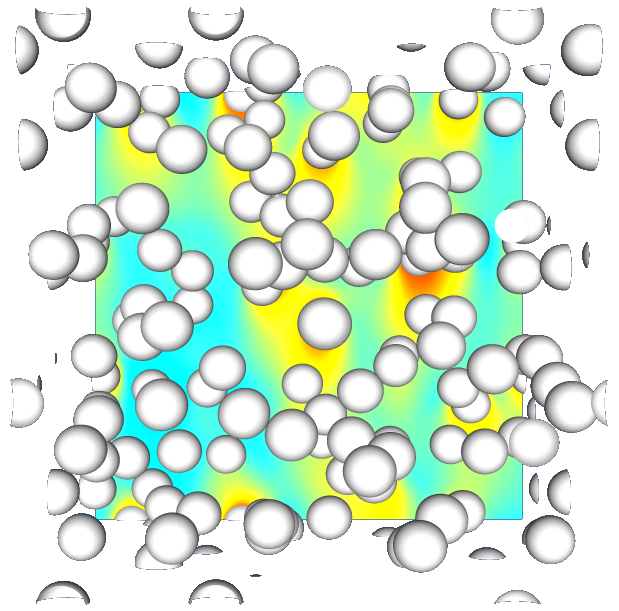
\includegraphics[height=4.5cm]{image/3D/P_PHI_5.png}
   %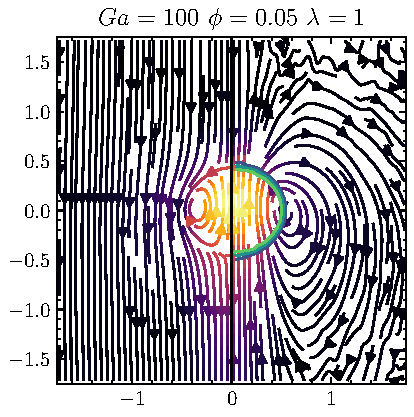
\includegraphics[height=5cm]{image/HOMOGENEOUS/Stream/Stream_PHI_5_Ga_100_l_1.pdf}
   %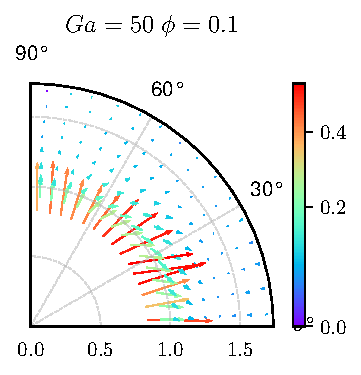
\includegraphics[height=4.5cm]{image/HOMOGENEOUS/fDrop/F_mu_r_1_0_Ga_50_PHI_0_1.pdf}
  \end{center}
  \caption{Buyancy driven motion of 125 droplets.}%Nearest-particle average of the fluid velocity. (left): streamlines in a fixed frame of reference, (right): streamline in the drop reference frame.}
  %(left) DNS of a buoyant emulsion with finite size 125 droplets using volume of fluid method.
  %(middle) Reconstruction of the nearest particle averaged eulerian velocity field.
  %(right) Reconstruction of the nearest particle averaged center of mass acceleration field.}
  \label{fig:tower}
\end{figure}
\bibliography{Bib/bib_bulles.bib}
\end{document}
%%%%%%%%%%%%%%%%%%%%%%%%%%%%%%%%%%%%%%%%%%%%%%%%%%%%%%%%%%%%%%%%%%%%%%%%%%%%%%%%%%%%%%%%%%%%%%%%%%%%%%%
